%!TEX root = ../report.tex

\chapter{Evaluation and results}
\section{Densenet}

%\section{Status}
%\begin{itemize}
% \item Coarse grid search with flatten -- Done
% \item Avg vs flatten pooling -- to analyze
% \item Growth rate analysis -- to analyze
% \item Std per dense block -- to analyze
% \item total number of parameters -- to analyze
% \item Finer grid search -- Next
% \item Compression and reduction -- to analyze
% \item Dropout -- to analyze
% \item Monte Carlo dropout
% \item Nb\_filter analysis --running
% \item Batch size -- to analyze
% \item optimizer and learning rate -- running only adadelta with various learning rates, takes too long otherwise. Even for that evalating for lower learning rates does not make sense so they are being run highest to lowest, 
% can be stopped from evaluating if the auc dips as expected.
% \item FINAL grid search -- TBD
%\end{itemize}

In Densenet each layer connects to every layer in a feed-forward fashion. 
With the basic idea to enhance the feature propagation, each layer of Densenet blocks takes the feature-maps of the previous stages as input.  

\begin{figure}[h]
\centering
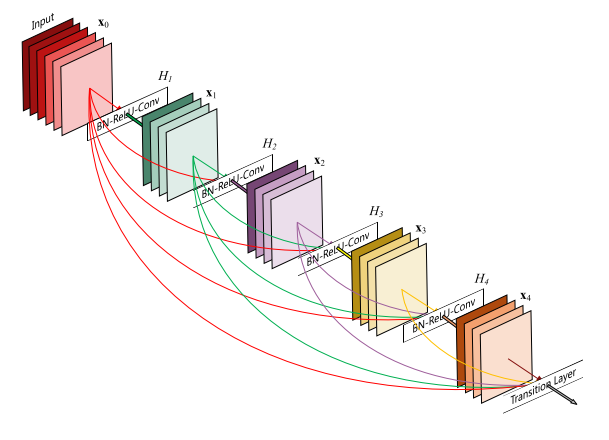
\includegraphics[width=0.5\textwidth]{images/densenet/densenet.png}
\caption{\label{fig:densenet}Densenet structure.}
\end{figure}
\flushbottom
\newpage

\subsection{Best hyper-parameters search spaces}
Hyper-parameters are those parameters whose values are set before the training, unlike other parameters whose values are learned during the training. 
For example learning rate, batch size. \cite{wikihyper}

\subsubsection{Parameters of Densenet}
\begin{itemize}
  \item \textbf{Growth rate}: Number of filters to add per dense block. Growth rate regulates how much information is contributed by each layers to the global state. 
  Global state is the collective knowledge of the network, that is the state of the previous layers are flown into each layer in form of feature-maps, 
  which is considered as global state. Each layer adds k more feature-maps to the current state, when growth rate is k.

  \item \textbf{Nb\_filter}: initial number of filters. -1 indicates initial number of filters will default to 2 * growth\_rate.

  \item \textbf{Nb\_layers\_per\_block}: number of layers in each dense block. Can be a -1, positive integer or a list. If -1, calculates nb\_layer\_per\_block from the network depth. 
  If positive integer, a set number of layers per dense block. If list, nb\_layer is used as provided. Note that list size must be nb\_dense\_block.

  \item \textbf{Depth}: number or layers in the DenseNet.

  \item \textbf{Nb\_dense\_block}: number of dense blocks to add to end.

  \item \textbf{Bottleneck Layers}: To improve computation efficiency a bottleneck layer with 1x1 convolution is introduced before each 3x3 convolution layers. 
  \item \textbf{Compression}: Reduces the feature maps in transition layers and makes the model more compact and computationally efficient.
\end{itemize}



\subsubsection{Other hyper-parameters}
Apart from the densenet there are other general hyper-parameters such as learning rate, batch size for training, optimizer. 


\subsubsection{Grid search strategy}
Since there are lot of parameters, practically, infinite test cases might be designed. To keep the grid search focused and less computationally expensive it makes sense to 
first search for coarser grid of parameters rather than very fine ones. When and if a bracket of parameters are shortlisted which works better than others, the finer parameter
search will be performed only specific to those range of parameters and not the whole grid.

\subsection{Analysis}

\subsubsection{Coarse grid search on Densenet hyper-parameters}
For the estimation of the best performing parameters of Densenet for the branches of the Siamese, first a coarse grid search is been performed with 
\begin{itemize}
 \item Layers per block are chosen among 2,3,4,5,6. For single dense block evaluation goes up-to 12 layers (per block). 
 \item Each network has been evaluated for growth rates of 12,18,24,30. %6, 36 excluded as they are too thin and too thick respectively. 
 \item Different dense block sizes of 1,2,3,4.  
 %\item Not all the possible combinations has been evaluated as quite extensive as possible
 \item The basic idea here is to narrow down the possible network sizes from the Densenet parameters perspective. There are other parameters but number of dense block, 
 growth rate and layers per block are three main parameters which controls the architecture/size of the network the most.
 \item The parameters compression/reduction and bottleneck are set 0.5 and False respectively. For more fine grained analysis the compression and bottleneck parameters might be evaluated. 
 \item nb\_filter values are fixed at 16 for this test
 \item The parameter classes are set to 2, where class 1 for matching patches and 0 for not-matching patches.
 \item 96,96 is the input image dimensions. And input is two channel. So depending on local setting of the keras, “channel-first” or “channel-last” suitable input\_shape is 
 chosen automatically as  2,96,96  or 96,96,2 respectively.
 \item The learning rate used for the test was is 0.07 and Adadelta as optimizer. Best performing combination from Densenet Siamese analysis.
 \item Dropout for Densenet used as 0.2 to handle regularization.
 \item Epochs are different for different architectures to ensure that the networks are able to train decently %95\% training accuracy. 
 \item Some of this values needs to be further evaluated as well, how ever current values were obtained using some of manual tuning and assumed to be a decent starting point.
 \item Flatten is used as pooling at the end of the Densenet, it is introduced by this work which replaces the Globalaveragepooling step with a flatten. This causes increase 
 in parameters overall though.
 \item Binary\_crossentropy loss function with sigmoid activation function used for the binary classification, this final layer acts as the binary classifier.
 \item In all the cases the networks are being trained from scratch. The weights value None ensures that no previously trained weights are used.
\end{itemize}

\subsubsection{Coarse grid search parameters summary}
\begin{flushleft} {Fixed hyper-parameters}
\begin{itemize}
 \item Nb\_filter: 16
 \item Subsample initial block: True
 \item Weights : None
 \item Dropout rate : 0.2
 \item Include top : True
 \item Compression : 0.5
 \item Bottleneck : False
 \item Transition pooling : max
\end{itemize}
\end{flushleft}

\begin{flushleft}{Varying hyper-parameters}
 \begin{itemize}
  \item \textbf{Nb\_layers\_per\_block}:
  \begin{itemize}
   \item \textbf{One dense block architecture (nb\_dense\_block=1):}\\
   '2', '4', '6', '8', '10', '12'
   \item \textbf{Two dense block architecture (nb\_dense\_block=2):}\\
   '2-2', '4-4', '6-6'
   \item \textbf{Three dense block architecture (nb\_dense\_block=3):}\\
   '2-2-2', '4-4-4', '6-6-6'
   \item \textbf{Four dense block architecture (nb\_dense\_block=4):}\\
   '2-2-2-2', '4-4-4-4', '6-6-6-6'
  \end{itemize}
 \item \textbf{Growth rate}:
  \begin{itemize}
  \item Thin layers: 12, 18    
  \item Thick layers: 24, 30    
 \end{itemize}
 \item \textbf{Pooling}:
 \begin{itemize}
  \item Flatten
  \item Average (avg)
 \end{itemize}  
 
\end{itemize}
 
\end{flushleft}

\flushbottom
\newpage

\subsubsection{Architecture analysis}
\begin{figure}
    \centering
    \begin{subfigure}[b]{0.4\textwidth}
        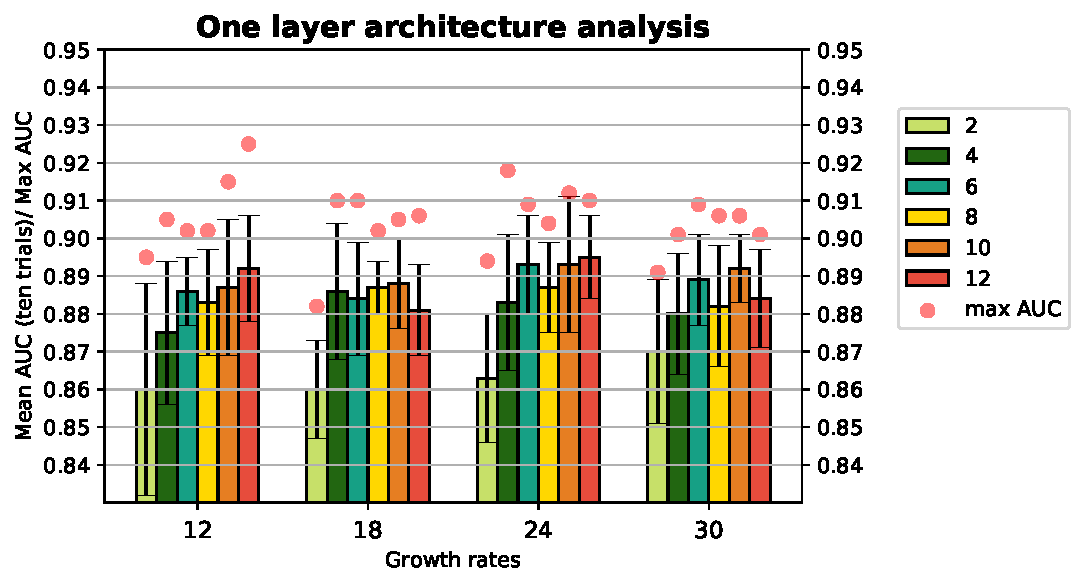
\includegraphics[width=\textwidth]{images/densenet/simple/densenet_simple_single_layer_bar}
        \caption{Single layer }
        \label{fig:densenet_simple_single_layer_bar}
    \end{subfigure}
    ~ %add desired spacing between images, e. g. ~, \quad, \qquad, \hfill etc. 
      %(or a blank line to force the subfigure onto a new line)
    \begin{subfigure}[b]{0.4\textwidth}
        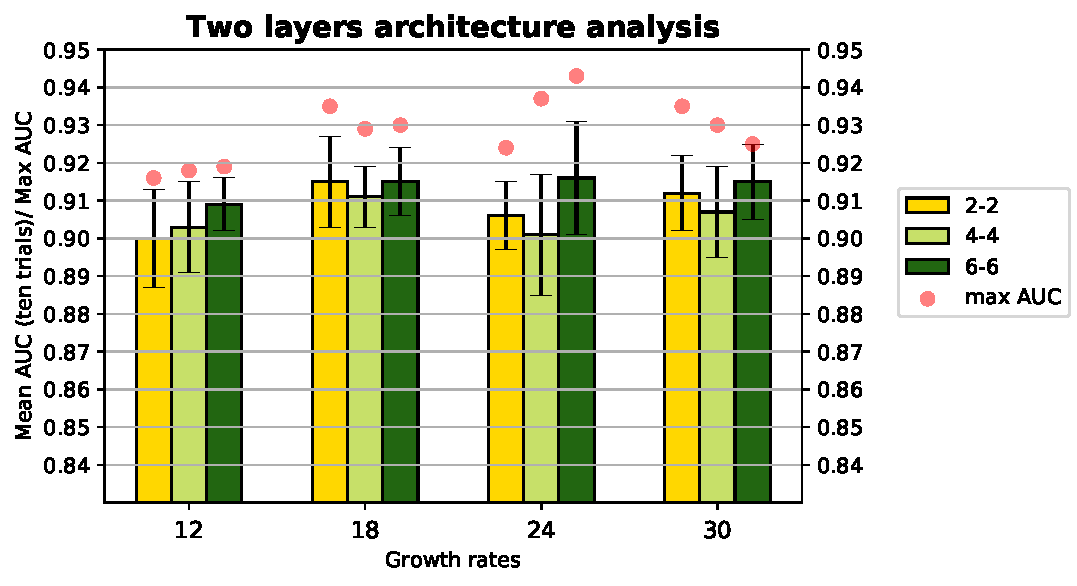
\includegraphics[width=\textwidth]{images/densenet/simple/densenet_simple_double_layer_bar}
        \caption{Two layers}
       \label{fig:densenet_simple_double_layer_bar}
    \end{subfigure}    
    \quad
    \centering
    \begin{subfigure}[b]{0.4\textwidth}
        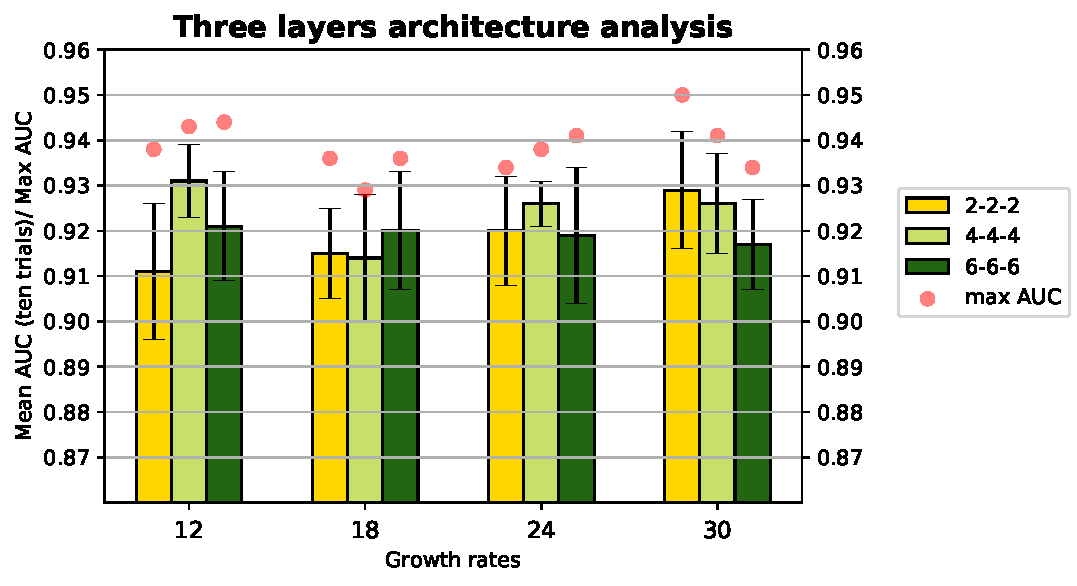
\includegraphics[width=\textwidth]{images/densenet/simple/densenet_simple_three_layer_bar}
        \caption{Three layers }
        \label{fig:densenet_simple_three_layer_bar}
    \end{subfigure}
    ~ %add desired spacing between images, e. g. ~, \quad, \qquad, \hfill etc. 
      %(or a blank line to force the subfigure onto a new line)
    \begin{subfigure}[b]{0.4\textwidth}
        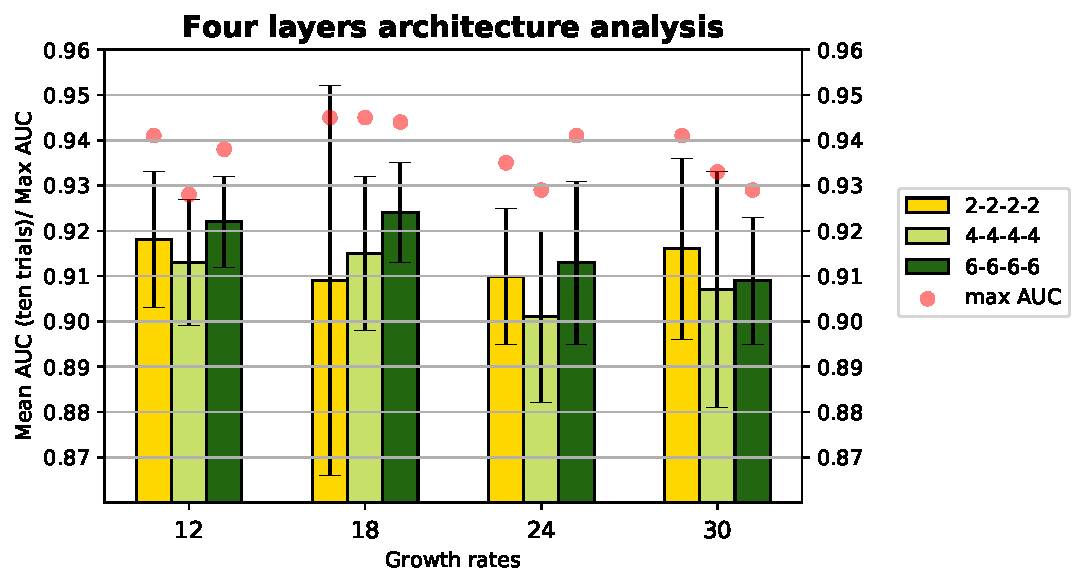
\includegraphics[width=\textwidth]{images/densenet/simple/densenet_simple_four_layer_bar}
        \caption{Four layers}
       \label{fig:densenet_simple_four_layer_bar}
    \end{subfigure} 
    \caption{Densenet two-channel architecture analysis}
    \label{fig:dense_arch_1}
\end{figure}  

\textbf{Conclusion}
\begin{itemize}
 \item It is clear that 4 blocks and 3 blocks network is performing better than the 1 and 2 blocks network
 \item Original paper also used 3 and 4 blocks densenet, so shall we.
\end{itemize}

\subsubsection{Pooling avg vs flatten}
The type of pooling used at the end of the network also determines the size of the total parameter size and also affects the generalization of the data. The original paper has used global average pooling. 
For the avg pooling comparison the 3 layer and 4 layer Densenet blocks have been compared. The results are as follows. It is observed that between the three layer and four layers Densenet the three layers
one is performing better. Overall the avg pooling is resulting in smaller total network parameters also the better results.

\begin{figure}
    \centering
    \begin{subfigure}[b]{0.4\textwidth}
        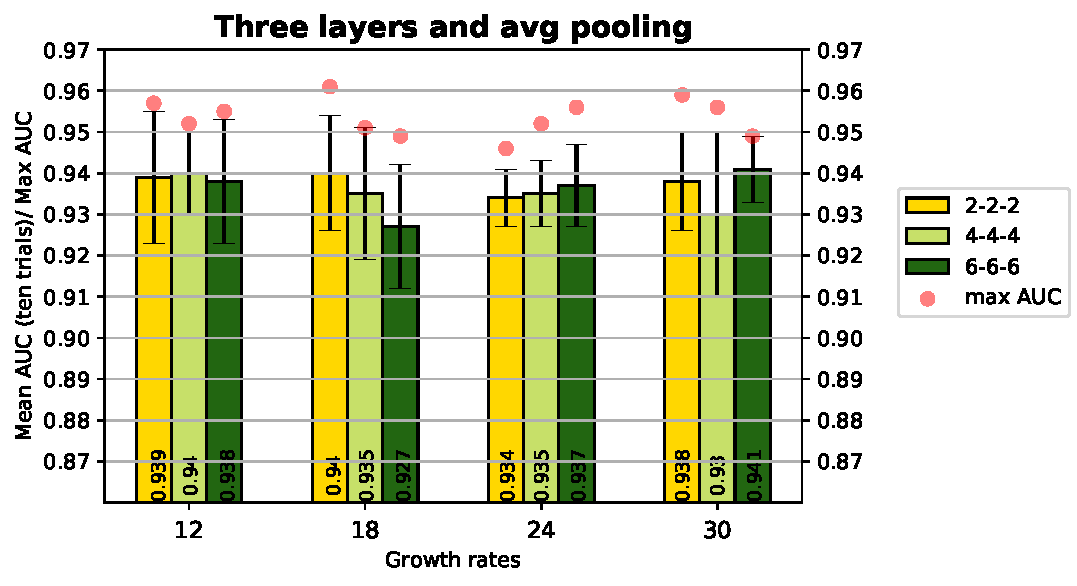
\includegraphics[width=\textwidth]{images/densenet/simple/densenet_simple_three_layer_avg_bar}
        \caption{Three layers avg pooling }
        \label{fig:densenet_simple_three_layer_avg_bar}
    \end{subfigure}
    ~ %add desired spacing between images, e. g. ~, \quad, \qquad, \hfill etc. 
      %(or a blank line to force the subfigure onto a new line)
    \begin{subfigure}[b]{0.4\textwidth}
        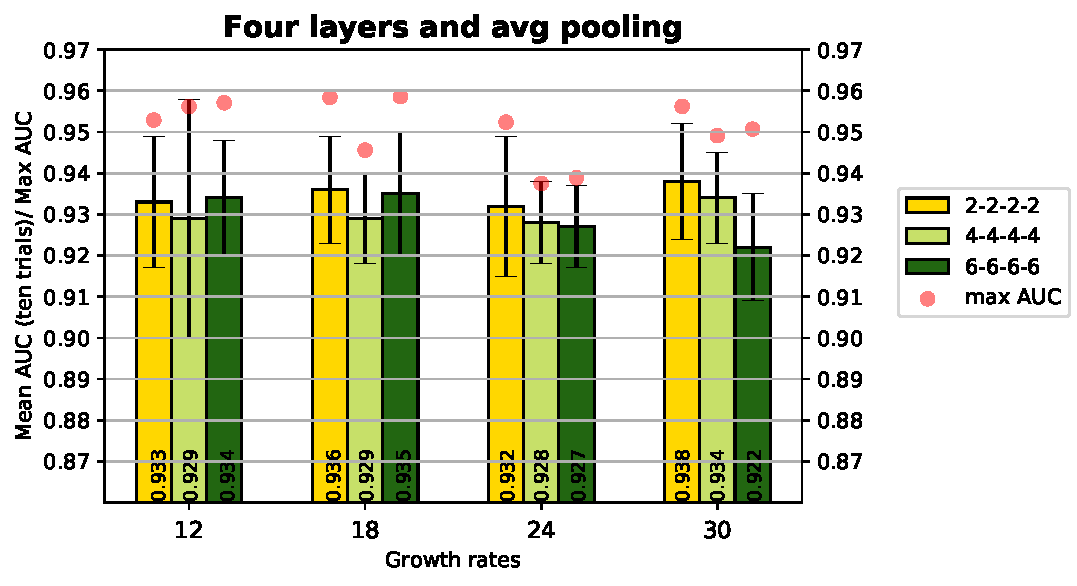
\includegraphics[width=\textwidth]{images/densenet/simple/densenet_simple_four_layer_avg_bar}
        \caption{Four layers avg pooling}
       \label{fig:densenet_simple_four_layer_avg_bar}
    \end{subfigure}        
    \caption{Densenet two-channel avg pooling analysis}
    \label{fig:dense_avg_pooling_1}
\end{figure}

For a comparitive analysis between the flatten and average pooling the mean AUCs are compared for each of the growth rates and for three layers Densenet( 2-2-2, 4-4-4, 6-6-6). Results are displayed in the figure below.
\begin{figure}[h]
\centering
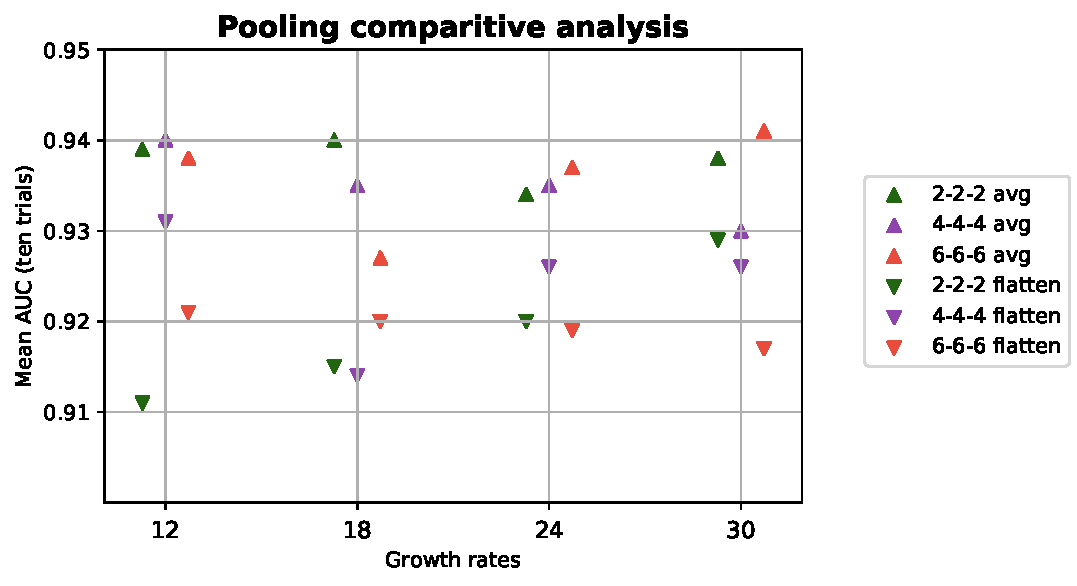
\includegraphics[width=0.5\textwidth]{images/densenet/simple/densenet_simple_three_layer_pooling_compare}
\caption{\label{fig:densenet_simple_three_layer_pooling_compare}Average vs flatten pooling}
\end{figure}

Here, the triangles up represents the mean AUC obtained using average pooling for each of the test cases. And triangle down represents flatten pooling. While the mean AUC for each of the three layers Densenet
architectures have been grouped according to four different growth rates. So the x axis of the graph shows growth rates 12, 18, 24 and 30. The y axis represents the mean AUC obtained from 10 trials. Each time 
the network, with the same settings, were trained from the scratch.
From figure \ref{fig:densenet_simple_three_layer_pooling_compare} it is clearly seen that the average pooling produces better results than using flatten, in all the cases. 

\subsubsection{Nb\_filter analysis}
Initial number of filters. 8,16,32,64 are being evaluated here. Also a comparison between mean AUCs obtained from growth rate 18 and 30 is done under this analysis. Ten evaluations of each test cases has been done.

\begin{figure}[ht]
\centering
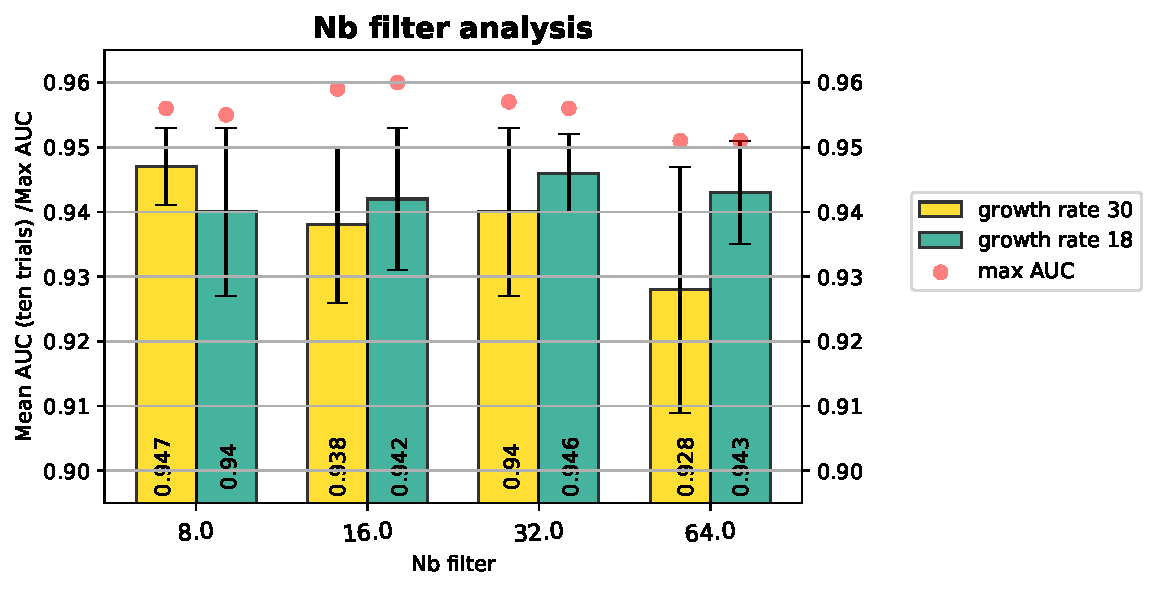
\includegraphics[width=0.5\textwidth]{images/densenet/simple/densenet_simple_nb_filter}
\caption{\label{fig:densenet_simple_nb_filter}Nb filter size analysis analysis}
\end{figure}

\textbf{Conclusion}
With change in nb filter size the mean AUC varies alot for higher growth rate such as 30, for growth rate 18 it does not vary so much. For growth rate 30 the nb filter 8 has the best mean AUC. 
For growth rate 18 the nb filter 32 has the best mean AUC. Overall growth rate 30 with nb filter 8 and growth rate 18 with nb filter 32 are the best combinations.
\subsubsection{Reduction and bottleneck analysis}
This analysis is for evaluating the effect of different reduction rates and the effect of bottleneck. So the mean AUC was recorded for 10 trials for each of the reduction values 0, 0.2, 0.3, 0.5, 0.7. This is a rather coarser 
search space. But each of them were also evaluated with bottleneck, the effect of varying values of reduction and with/without bottleneck has been evaluated. The results are displayed in the figure below. 
\begin{figure}[ht]
\centering
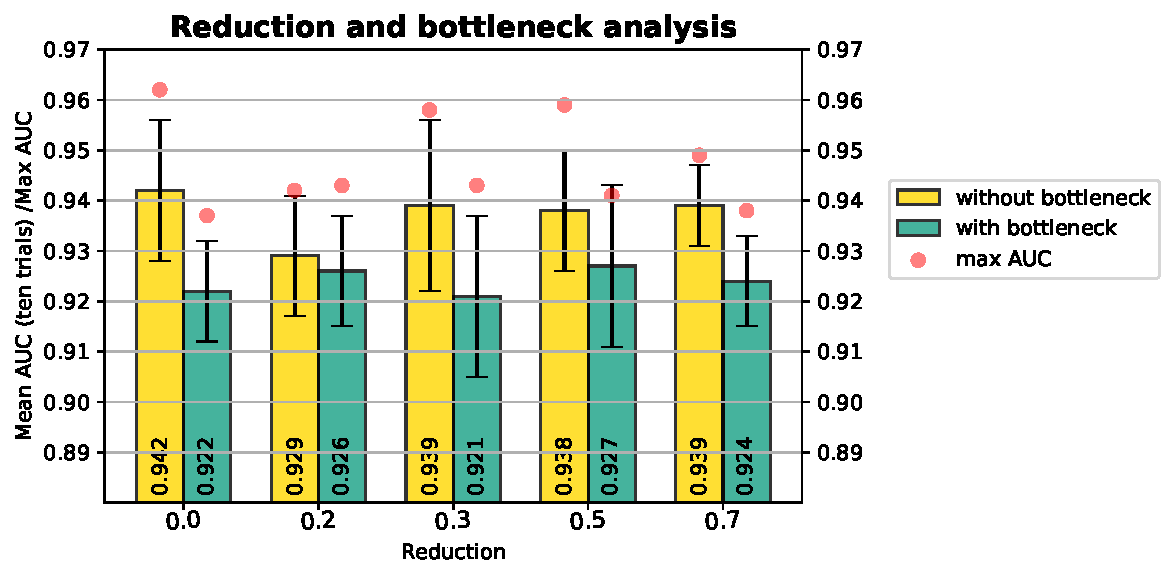
\includegraphics[width=0.5\textwidth]{images/densenet/simple/densenet_simple_reduction_bottleneck}
\caption{\label{fig:densenet_simple_reduction_bottleneck}Reduction and bottleneck analysis}
\end{figure}

\textbf{Conclusion}
\begin{itemize}
 \item The effect of the bottleneck layer is rather limiting the generalization of the network. So it seems like without bottleneck should be used for future evaluations.
 \item The performance without reduction is best as expected, how ever main purpose of the reduction is to decrease the number of total parameters. So in that sense, mean AUC obtained of reduction 0.3, 0.5 and 0.7 are all very 
 good even though the size of the total parameters is much lower. So values around 0.7 will be used for the final grid search. In the original implementation 0.5 is the default value used.
 \item TODO: the value for 0.2 is rather unexpected. The value was expected to be lesser than without reduction and with very high reduction.
\end{itemize}

\subsubsection{Total parameters analysis}
\begin{itemize}
 %\item How ever as the number of dense blocks keeps getting higher the non-trainable parameters also gets higher. So 4 blocks dense net has most number of non-trainable parameters.
 \item For the comparison 2, 2-2, 2-2-2, 2-2-2-2 blocks parameter sizes are compared below, all recorded for growth rate 18.
 \item FLATTEN VS AVG POOLING and effect
 \item Reduction effect
\end{itemize}

\subsubsection{Standard deviation across blocks}
TODO

\subsubsection{Dropout analysis}
Densenet dropout: 10 evaluations each \\
\begin{figure}[ht]
\centering
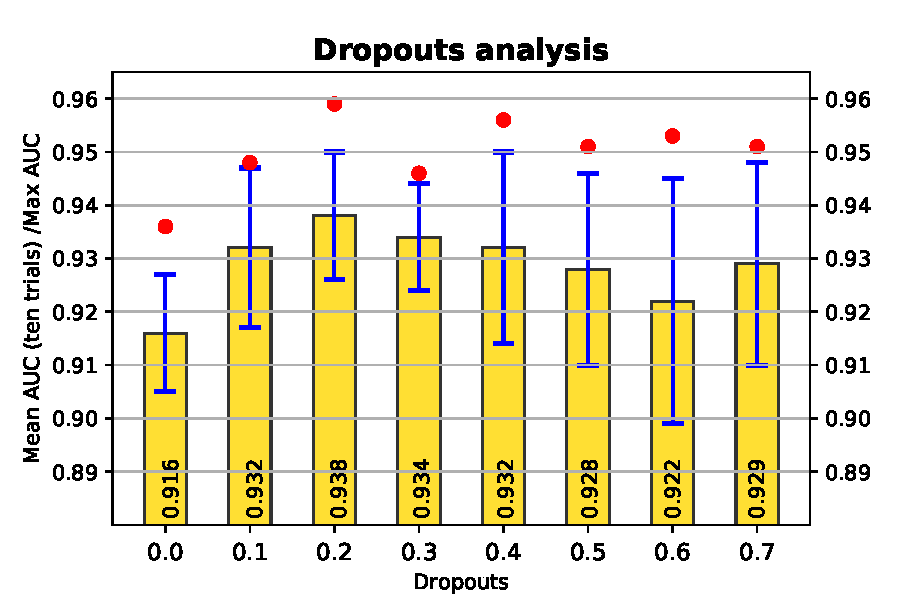
\includegraphics[width=0.5\textwidth]{images/densenet/simple/densenet_simple_dropout}
\caption{\label{fig:densenet_simple_dropout}Dropouts analysis}
\end{figure}

It is observed that the 0.2 dropout configuration has obtained the highest mean AUC. The other values with lesser dropouts or greater dropouts are all gradually decreasing as they go further from the peak (0.2). 
With exception of the mean AUC obtained with 0.7 dropouts.
\flushbottom
\newpage

\subsubsection{Batch size analysis}
If the batch size is too low then it takes more time and after a certain size it does not train well too.\\
If the batch size is very big then it may train faster but they generalize lesser as they tend to converge to sharp minimizers of the training function.
TODO add source (https://arxiv.org/abs/1609.04836) 

\begin{figure}[ht]
\centering
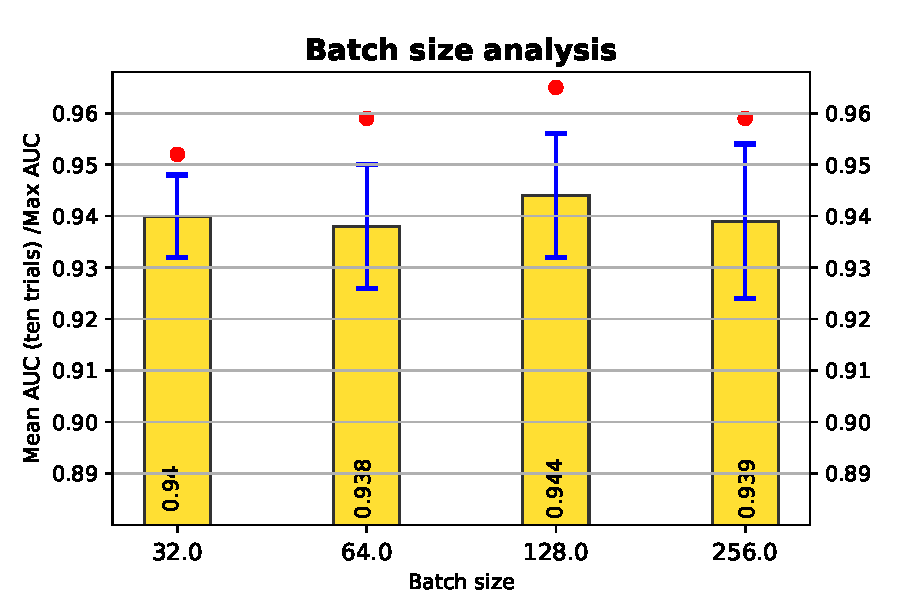
\includegraphics[width=0.5\textwidth]{images/densenet/simple/densenet_simple_batchsize}
\caption{\label{fig:densenet_simple_batchsize}Batch size analysis}
\end{figure}
  
\textbf{Conclusion}
From the figure \ref{fig:densenet_simple_batchsize} it is concluded that the batch size of 128 works the best. 
\flushbottom
\newpage

\subsubsection{Learning rate and optimizer analysis}
For this analysis the Adadelta optimizer is used only. This is based on the intuition that was formed during the Densenet Siamese evaluation.

\begin{figure}[ht]
\centering
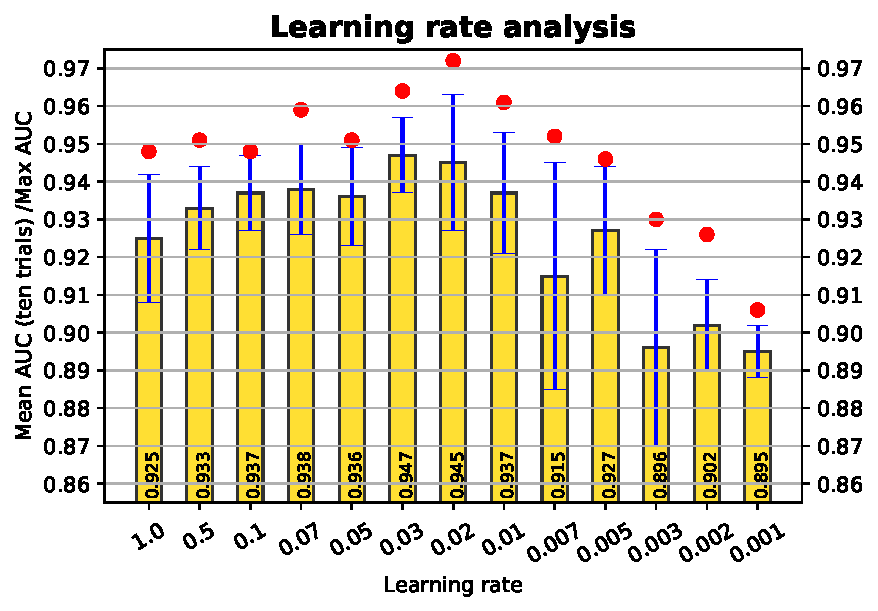
\includegraphics[width=0.5\textwidth]{images/densenet/simple/densenet_simple_learning_rate}
\caption{\label{fig:densenet_simple_learning_rate}Learning rate analysis}
\end{figure}

\textbf{Conclusion} 
From figure \ref{fig:densenet_simple_learning_rate} it is observed that the mean AUC with the learning rate 0.03 is slightly higher than the others. While one of the evaluation with 0.02 learning rate has 
obtained the maximum AUC of 0.972. So the best learning rate is considered to lie around the 0.02-0.03 region.


\subsubsection{Hyper-parameters for final grid search}

\begin{itemize}
 \item Growth rate, in the original paper, authors have mentioned that without bottleneck and compression the general trend is to use as high as possible growth rate. For the Imagenet, they have used growth rate 
 upto 40. For all their experiments they have evaluated growth rates from 12 to 40. Since we do not have so much of data, we will evaluate the finer grid search with growth rates of 12(thin), 18 and 30(thick). 
 \item Layers per block 2-2-2 it has very consistant performance in terms of mean AUC and also able to score high max AUC. It could have been possible to do architecture searches for 3 dense block architectures 
 with layers per block close to 2-2-2, for example 2-3-3 etc. But then the search grid will be very big.
 \item Bottleneck no
 \item Reduction 0 and 0.5
 \item Nb filter for 12, 18 growth rates use 32 and for growth rate 30 use 8.
 \item Dropout 0.2
 \item Adadelta with 0.03 learning rate
 \item Batch size 128
\end{itemize}

The result is displayed in the table \ref{table:final_densenet_results}. Here the multi dimension search space and associated results are displayed. Three architectures 2-2-2, 4-4-4 and 6-6-6 are evaluated for
all three growth rates 12, 18, 30 and also for Reduction 0.5 and without Reduction. In the table \ref{table:final_densenet_results} the growth rate is displayed as Gr. and Reduction is displayed as R for space 
constraint.

\definecolor{Gray}{gray}{0.8}

\begin{center}
\begin{table}
 \begin{tabular}{|c|l|cc|cc|cc|}\hline \hline
  \multirow{3}{*}{Gr.} & \multicolumn{1}{c|}{\multirow{3}{*}{Metrics}} & \multicolumn{6}{c|}{Layers per block}  \\ \cline{3-8}
  & & \multicolumn{2}{c|}{2-2-2} & \multicolumn{2}{c|}{4-4-4} & \multicolumn{2}{c|}{6-6-6}\\ \cline{3-8}
  & & R=0 & R=0.5 & R=0 & R=0.5 & R=0 & R=0.5 \\ \hline \hline
  %\rowcolor{Gray}
  \multirow{4}{*}{12} & Mean AUC & \cellcolor{Gray}0.95 & \cellcolor{Gray}0.944 & \cellcolor{Gray}0.95 & \cellcolor{Gray}0.95 & \cellcolor{Gray}0.947 & \cellcolor{Gray}0.945 \\ %\cline{2-8}
   & Std & 0.011 & 0.015 & 0.009 & 0.01 & 0.008 & 0.008 \\ %\cline{2-8}
   & Max AUC & 0.97 & 0.97 & 0.963 & 0.965 & 0.963 & 0.955 \\ 
   & Total Parameters & 55,529 & 30,163 & 159,473 & 87,629 & 317,561 & 176,535 \\ \hline 
   %\rowcolor{Gray}
  \multirow{4}{*}{18} & Mean AUC & \cellcolor{Gray}0.952 & \cellcolor{Gray} 0.955 & \cellcolor{Gray} 0.951 & \cellcolor{Gray} 0.944 & \cellcolor{Gray} 0.948 &  \cellcolor{Gray} 0.938 \\ %\cline{2-8}
   & Std & 0.008 & 0.009 & 0.005 & 0.011 & 0.006 &  0.014 \\ %\cline{2-8}
   & Max AUC & 0.967 & 0.966 & 0.956 & 0.963 & 0.956 & 0.955 \\ 
   & Total Parameters & 96,785 & 51,430 & 308,369 & 168,671 & 640,481 & 355,860 \\\hline 
   %\rowcolor{Gray}
  \multirow{4}{*}{30} & Mean AUC & \cellcolor{Gray} 0.943 & \cellcolor{Gray} 0.948 & \cellcolor{Gray} 0.943 & \cellcolor{Gray} 0.944 & \cellcolor{Gray} 0.932 & \cellcolor{Gray} 0.941 \\ %\cline{2-8}
   & Std & 0.008 & 0.008 & 0.01 & 0.013 & 0.015 &  0.011 \\ %\cline{2-8}
   & Max AUC & 0.959 & 0.964 & 0.96 & 0.962 & 0.948 & 0.953 \\ 
   & Total Parameters & 160,001 & 82,162 & 650,873 & 355,949 & 1,473,665 & 822,276 \\ \hline
  \hline
 \end{tabular}
 \caption{Final grid search results}
\label{table:final_densenet_results}
\end{table}

\end{center}

%Divide this into three tables as well for densenet for fc + normal
%\begin{center}
% \begin{tabular}{||c c c c c c c c c c c c c c c c c||} 
% \hline\hline
% Layers & Growth\_rate & dense\_block & nb\_filter & dropout & reduction\_ & bottleneck & fc\_dropout & fc\_filter & Epochs & batch\_size & lr & optimizer & es\_patience & lr\_patience & batch\_size \\ [0.5ex] 
% \hline
% 0.608 & 0.854 & 0.881 & 0.902 & 0.934 & 3 & 0.608 & 0.854 & 0.881 & 0.902 & 0.934 & 3 & 0.608 & 0.854 & 0.881 & 0.902 & 0.934 \\ 
% \hline
% 0.608 & 0.854 & 0.881 & 0.902 & 0.934 & 3 & 0.608 & 0.854 & 0.881 & 0.902 & 0.934 & 3 & 0.608 & 0.854 & 0.881 & 0.902 & 0.934 \\
% \hline
%\end{tabular}
%\end{center}

%\flushbottom
%\newpage
\subsubsection{Conclusion}

\begin{itemize}
 \item The best result obtained has mean AUC of 0.955. This is with reduction 0.5, 2-2-2 layers per block and growth rate of 18. Normally it is observed that the 2-2-2 performance
 is very similar to that of 4-4-4, in fact slightly better. The performance of 6-6-6 is bit worse than the other too. 
 \item Though because of reduction the auc is observed to be slightly lower some times, some times it is higher than the without reduction result. But the size of the total parameters 
 of the network with Reduction(R)=0.5 is always close to half size of the equivalent network without Reduction. So that is always beneficial as it is less computationally expensive.
 \item In Matias's work it was also found that the simple two channel network better than the siamese network. Using Densenet it is also seen to be the truth.
\end{itemize}

\begin{figure}[ht]
\centering
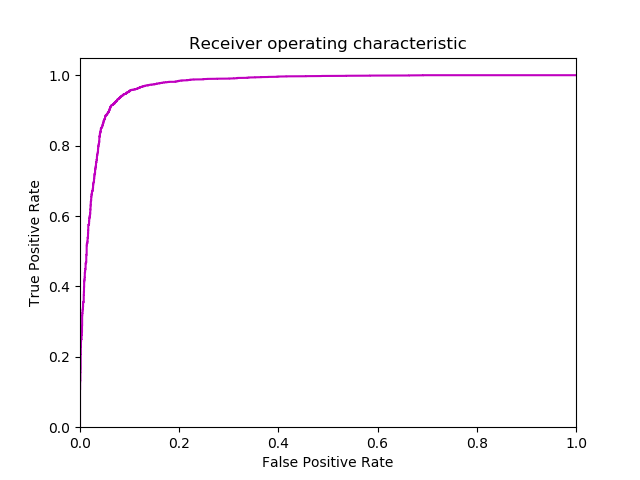
\includegraphics[height= 5cm]{images/densenet/densenet_two_channel_ninetysevenAUC}
\caption{AUC curve Overall best result in both densenet architectures 0.973 AUC (Single run)}
\label{fig:densenet_two_channel_ninetysevenAUC}
\end{figure}


\section{Comparitive analysis}
So the three network structure that were used, will be compared in this section, in terms of AUC value obtained. Time of execution, total parameters also by using the uncertainty calculated from the Monte Carlo 
drop out calculations. All our final models were trained with dropouts, as that was the best parameters set up for the network. 

\subsection{AUC comparison}
Densenet two channel has highest mean AUC(10 Trials) of \textbf{0.955}, std 0.009 with max AUC of 0.966. With total parameters of only 51,430. 
Densenet Siamese has highest mean AUC(10 Trials) of \textbf{0.921}, std 0.016, Max AUC, 0.95 With total parameters of only 16,725,485. This total parameter size is so large because of the multiplication of the flattened
feature map from each Densenet branch with fully connected layer of Siamese branch and following concatenation of the feature maps from both Densenet branches.
Contrastive loss with VGG-Siamese network have results of mean AUC (Ten trials) of \textbf{0.944} with std of 0.007 and highest AUC value in a single run as 0.951. With total parameter size of 3,281,840. Though another 
network structure has scored 0.943 mean AUC, std 0.006 and max AUC of 0.951 with total parameters size of 1,068,080. The difference between the two network is the size of the output of the fully connected layer, 2048 is 
the fully connected network output size for the bigger network, and for the smaller network that is 128. As an effect the total number of parameters are almost one third but the performance is almost same. 

\begin{center}
\begin{table}
\begin{tabular}{|c c c c c|} 
 \hline\hline
 Network & Mean AUC & Std & Max AUC & Total params\\ \hline
 Densenet two channel & 0.955 & 0.009 & 0.966 & 51,430\\
 Densenet Siamese & 0.921 & 0.016 & 0.95 & 16,725,485 \\
 Contrastive loss & 0.944 & 0.007 & 0.951 & 3,281,840\\ \hline \hline
 \end{tabular}
 \caption{Comparative analysis on the AUC and total number of parameters in the best performing networks.}
\label{table:comparative_auc_results}
\end{table}
\end{center}
